%% ----------------------------------------------------------------
%% Thesis.tex -- MAIN FILE (the one that you compile with LaTeX)
%% ---------------------------------------------------------------- 

% Set up the document
\documentclass[a4paper, 11pt, oneside]{Thesis}  % Use the "Thesis" style, based on the ECS Thesis style by Steve Gunn
\graphicspath{{Figures/}}  % Location of the graphics files (set up for graphics to be in PDF format)

% Include any extra LaTeX packages required
\usepackage[square, numbers, comma, sort&compress]{natbib}  % Use the "Natbib" style for the references in the Bibliography
\usepackage{verbatim}  % Needed for the "comment" environment to make LaTeX comments
\usepackage{vector}  % Allows "\bvec{}" and "\buvec{}" for "blackboard" style bold vectors in maths
\hypersetup{urlcolor=blue, colorlinks=true}  % Colours hyperlinks in blue, but this can be distracting if there are many links.

\usepackage{amsmath}
\usepackage{lmodern} %Do get the right font encoding
\usepackage{lipsum}

%\setlength{\parindent}{0.8cm}
%\setlength{\parskip}{0pt}
%% ----------------------------------------------------------------
\begin{document}
\frontmatter	  % Begin Roman style (i, ii, iii, iv...) page numbering

% Set up the Title Page
\title  {Clustering Player Behaviors in Data Streams using K-means in MapReduce}
\authors  {\texorpdfstring
            {\href{sigurdurm@gmail.com}{Sigurdur Karl Magnusson}}
            {Sigurdur Karl Magnusson}
            }
\addresses  {\groupname\\\deptname\\\univname}  % Do not change this here, instead these must be set in the "Thesis.cls" file, please look through it instead
\date       {\today}
\subject    {}
\keywords   {}

\maketitle
%% ----------------------------------------------------------------

\setstretch{1.3}  % It is better to have smaller font and larger line spacing than the other way round

% Define the page headers using the FancyHdr package and set up for one-sided printing
\fancyhead{}  % Clears all page headers and footers
\rhead{\thepage}  % Sets the right side header to show the page number
\lhead{}  % Clears the left side page header

\pagestyle{fancy}  % Finally, use the "fancy" page style to implement the FancyHdr headers


%% ----------------------------------------------------------------
% The "Funny Quote Page"
\pagestyle{empty}  % No headers or footers for the following pages

\null\vfill
% Now comes the "Funny Quote", written in italics
\textit{``Any intelligent fool can make things bigger, more complex, and more violent. It takes a touch of genius -- and a lot of courage -- to move in the opposite direction.''}

\begin{flushright}
Albert Einstein
\end{flushright}

\vfill\vfill\vfill\vfill\vfill\vfill\null
\clearpage  % Funny Quote page ended, start a new page
%% ----------------------------------------------------------------

% The Abstract Page
\chapter*{Abstract}
\addcontentsline{toc}{chapter}{Abstract}
\thispagestyle{plain}

\lipsum[1]

\clearpage  % Abstract ended, start a new page
%% ----------------------------------------------------------------

\setstretch{1.3}  % Reset the line-spacing to 1.3 for body text (if it has changed)

% The Acknowledgements page, for thanking everyone
\acknowledgements{
\addtocontents{toc}{\vspace{1em}}  % Add a gap in the Contents, for aesthetics

The acknowledgments and the people to thank go here, don't forget to include your project advisor\ldots

}
\clearpage  % End of the Acknowledgements
%% ----------------------------------------------------------------

\pagestyle{fancy}  %The page style headers have been "empty" all this time, now use the "fancy" headers as defined before to bring them back


%% ----------------------------------------------------------------
\lhead{\emph{Contents}}  % Set the left side page header to "Contents"
\tableofcontents  % Write out the Table of Contents

%% ----------------------------------------------------------------
\lhead{\emph{List of Figures}}  % Set the left side page header to "List if Figures"
\listoffigures  % Write out the List of Figures

%% ----------------------------------------------------------------
\lhead{\emph{List of Tables}}  % Set the left side page header to "List of Tables"
\listoftables  % Write out the List of Tables

%% ----------------------------------------------------------------
\setstretch{1.5}  % Set the line spacing to 1.5, this makes the following tables easier to read
\clearpage  % Start a new page
\lhead{\emph{Abbreviations}}  % Set the left side page header to "Abbreviations"
\listofsymbols{ll}  % Include a list of Abbreviations (a table of two columns)
{
% \textbf{Acronym} & \textbf{W}hat (it) \textbf{S}tands \textbf{F}or \\
\textbf{LAH} & \textbf{L}ist \textbf{A}bbreviations \textbf{H}ere \\

}

%% ----------------------------------------------------------------
\mainmatter	  % Begin normal, numeric (1,2,3...) page numbering
\pagestyle{fancy}  % Return the page headers back to the "fancy" style

% Include the chapters of the thesis, as separate files
% Just uncomment the lines as you write the chapters

% Chapter 1

\chapter{Introduction} % Write in your own chapter title
\label{Chapter1}
\lhead{Chapter 1. \emph{Introduction}} % Write in your own chapter title to set the page header

\section{Motivation}
We live in a world where data is being generated at an amazing rate everywhere around us. Data can describe characteristics of e.g. Internet activities, social interactions, user actions and behaviors in games, scientific experiments and measurements from different devices and sensor equipments. Amount of data that is being registered and logged around us is growing in volume and complexity and storing the data in large databases or in more commonly on-line storage model called cloud storage just gets cheaper and cheaper. We live in a world of data and we are just at the beginning. 

\null
% Now comes the "Funny Quote", written in italics
\textit{``Information is the oil of the 21st century, and analytics is the combustion engine.''}

\begin{flushright}
Peter Sondergaard, senior VP at Gartner
\end{flushright}

In digital games, data about in-game user interactions have been logged and behaviors analyzed since the first game came out. Analyzing the user experience and behaviors of players have mostly been done in laboratories in the past, both during game development and after game launch to see if the game was played as designed. Game designs have becoming increasingly complex in the recent years offering much more freedom to the players by increasing the number of actions available, items to interact with and on-line massive multi-player persistent worlds that continue to exist after a player exits a game \citep{Kim:2008Tracking, Drachen:2011Evaluating}. This complexity generates much more user-centric data than before and is increasingly challenging when evaluating game designs \cite{Pagulayan:2002UserDesign, Seif:2013GameAnalytics}. The user interactions being registered is called \textit{user telemetry} and is translated to \textit{game metrics} as referred in game development, providing detailed and objective numbers, e.g. total playtime, monsters killed, puzzles solved.

Collecting user's telemetry can give very detailed quantitative information on player behavior and using data mining techniques can supplement traditional qualitative approaches with large-scale behavioral analysis \citep{Yannakakis:2012}, for example show where users are getting stuck and finding actionable behavioral profiles \citep{Kim:2008Tracking, Drachen:2012, Drachen:2011Evaluating}. In the recent years user behavior analysis have in part been driven by the emergence of massive multi-player on-line (MMO) games and Free-to-Play (F2P) games which can have millions of users and objects that can form highly complex interactions. These game models, especially of persistent nature, are constantly monitoring users actions and their behaviors by driving their revenue with subscriptions or offer players to buy virtual items via micro transactions \citep{Kim:2008Tracking, Drachen:2011Evaluating, Fields:2011SocialGame, Seif:2013GameAnalytics}. 

One way of doing a behavioral analysis is use an unsupervised machine learning technique called clustering. Cluster analysis is a popular exploratory data mining technique that groups set of data objects together in a cluster that are more similar to each other than data objects in other groups \citep{Xu:2005Clustering}. Human beings categorizes or classifies a new object or a phenomenon based on similarity or dissimilarity of the object's descriptive features and is one of most primitive activies of humans \citep{Anderberg:1973ClusterAnalysis}. Clustering explores the unknown patterns of the data and provide compressed data representation for large-scale data. In computer games cluster analysis or behavioral categorization can find behavioral profiles that are actionable and give high valuable insights into the game development as well as increasing the monetization \cite{Drachen:2009Tomb, Mahlmann:2010Tomb}. 

Most clustering algorithms are designed for modern sizes of datasets where the whole data can fit into memory or allows few passes into a database (where each data object is read more than once). It can be very expensive analyzing large-scale datasets and to get answers efficiently then one needs to reduce the set of data to be analyzed, e.g. sample fewer players and have fewer features (dimensions) to be compared. Computations for large-scale data takes time and needs to be distributed to be able to complete in reasonable amount of time. Google's MapReduce programming model was introduced in 2004 \citep{Dean:2004} and allows automatic parallelization and distribution of computations on large clusters of commodity computers. Allowing programmers and researchers to easily implement highly scalable algorithms to process large amount of data using the MapReduce model without worrying about handling failures and distributing the data with a large amount of complex code. 

\section{Problem Statement}

{\addtolength{\leftskip}{5mm} How can clustering using incremental k-means find general player behaviors in large-scale behavioral game data in reasonable time? \par}

Considering the massive size of user telemetry data being logged and processed, the complexity of game designs there is a knowledge gap when it comes to analyzing such large-scale data efficiently. Number of players are increasing and the complexity of player-game and player-player interactions grows exponentially. One of the largest massive multi-player on-line role-playing game (MMORPG) \textit{World of Warcraft} has a population of around 12 million users where players live in a persistent world and can create many millions of different interactions in the game. 

User telemetry from games can arrive in daily chunks and need to be processed incrementally (in mini batches). There is a need for algorithms that can process massive amount of data that doesn't fit in a computer memory to extracts knowledge in a reasonable time. K-means algorithm can find clusters of behaviors implemented in the MapReduce framework by processing the data in parallel and thus is highly scalable where running time increases linearly with the size of the input. 

Our goal with this project is to implement a scalable clustering algorithm to find the general behaviors in a specific real life game dataset in collaboration with GameAnalytics (GA) \citep{GA2013}. The goal is not to implement a complete product but an algorithm that provides information about the general player behavioral profiles for a specific game and support GA to further develop a product which is easily applied to future games. 

The success criteria of this project is:
\begin{itemize}
\item A scalable k-means clustering algorithm finding clusters describing the general behaviors of a real life game dataset provided by GameAnalytics.
\item The general behaviors found must be intuitively interpretable and actionable to game developers.
\item The algorithm must be able to process incrementally cluster daily arriving chunks of game metric data.
\end{itemize}

GameAnalytics is Software as a Service (SaaS) start-up, a data and analytics engine for game studios with its headquarters located in Copenhagen. Analyzing large quantities of game metric data that needs to be processed efficiently returning actionable results to aid game design and development. 

\section{Method}
TODO
A short description of the methods

\lipsum[2]

\section{Contributions}
TODO
Description of the contributions made in the project

\lipsum[3]


\section{Project Outline}
References are cited by index in the bibliography and are in order of appearance, e.g. [2] is a citation number two that is referenced in the thesis. Referring to other sections is by the number of that section, e.g. 4.1.2.

The organization of the thesis is as follows: 
\begin{itemize}
\item \textbf{Chapter 2 - Background} Describes a short background theory about clustering player behaviors and the MapReduce framework for large-scale data parallel processing.
\item \textbf{Chapter 3 - Related Work} Overview of related and recent work regarding clustering player behaviors and large-scale data with k-means as focus.
\item \textbf{Chapter 4 - Methodology} Our design and implementation work is described; Description of the real game dataset and selection of features, the k-means algorithm in MapReduce and the experimental set-up.
\item \textbf{Chapter 5 - Results} Results and observations from experiments are explained.
\item \textbf{Chapter 6 - Conclusions} Conclusions are drawn from the study including future research.
\end{itemize}
 % Introduction

% Chapter 2

\chapter{Background Theory} % Write in your own chapter title
\label{Chapter2}
\lhead{Chapter 2. \emph{Background Theory}} % Write in your own chapter title to set the page header


\section{Player Behaviour}
\subsection{Game Metric}
\subsection{Features}
\section{Clustering}
\subsection{K-Means}
\subsection{Streaming and Data Streams}
\section{Map-Reduce and Hadoop}
 % Background Theory 

% Chapter 3

\chapter{Related Work} % Write in your own chapter title
\label{Chapter3}
\lhead{Chapter 3. \emph{Related Work}} % Write in your own chapter title to set the page header

Clustering player behaviors and processing large data sets have been researched actively in the recent years. In our work we find the general player behaviors in a the case study using k-means clustering algorithm in the MapReduce framework for high scalability and parallel processing of large-scale data. The behavior of the data can change from day to day like when dealing with an endless stream of data is also discussed. In subsequent sections some of the recent and related work are given a short introduction.

\section{Clustering Player Behaviors}
Many researches have been done on clustering and predicting player behaviors over the last years to get a better understanding which kind of user behaviors are to be found when playing a game that can be actionable for game developers \citep{Marsh:2006Continuous, Missura2009Player, Thurau:2009SVIM, Drachen:2011Evaluating, Drachen:2012}. User behavior analysis has becoming increasingly popular in the recent years because of rise of the free-to-play (F2P) genre games in \textit{Facebook} and \textit{Google Play} where populations can be in millions creating complex game interactions \citep{Kim:2008Tracking, Drachen:2011Evaluating}. Playing these games are free and many are of persistent nature where the world in the game continues when a player exits. To be profitable these games drive their revenue via micro transactions, e.g. players buying upgrades or virtual items in game for real money \citep{Kim:2008Tracking, Drachen:2011Evaluating, Fields:2011SocialGame, Seif:2013GameAnalytics}. Major game publishers have also been collecting and analyzing large scale of behavior telemetry data but details of their methods are kept confidential \citep{Zoeller:2010, Yannakakis:2012}. Most available research work is case-based where a specific algorithm is applied to a specific game and commercial game data sets has only become accessible recently for academic researchers \citep{Yannakakis:2012}.

Predicting player behavior in a major commercial game Tomb Raider: Underworld (TRU) was presented in a study of Drachen et al. \citep{Drachen:2009Tomb}. Authors classified 1365 players in a moderate data set into four user behavioral groups using six statistical gameplay features based on core game design as inputs of an emergent self-organizing map to identify dissimilar behavior clusters. Behavior profiles covering 90 percent of the users in the dataset were labeled in game terminology usable for game designers. Mahlmann et al. \citep{Mahlmann:2010Tomb} did a follow up on the research using eight gameplay features and classified behavior of 10,000 players. The authors presented also how to predict behavior based on early play analysis, a popular topic which can be used to prevent churn (attrition) \citep{Fields:2011SocialGame}.

Analyzing social groups in the highly popular Massively Multiplayer Online Role-Playing Game (MMORPG) World of Warcraft was done by Thurau and Bauckhage \citep{Thurau:2010WoW}. They analyzed how groups (guilds) evolve over time from both American and European based guilds. Their paper is the first study analyzing such amount of data in a MMORPG, analyzing large-scale data gathered on-line from 18 million players belonging in 1.4 million groups over a period of 4 years. Convex-Hull Non Negative Matrix Factorization (CH-NMF) \citep{Thurau:2009SVIM} technique was applied to the data to find the extremes rather than averages and the results show  no significant cultural difference in formation processes of guilds from either the US or the EU. Interpretability of CH-NMF was more distinguishable and representing archetypal guilds than the more conventional clustering method k-means that represent the cluster centroids with similar characteristic.

Drachen et al. \citep{Drachen:2012} did a clustering analysis for two major commercial games applied to large-scale of high-dimensionality player behavior telemetry. K-means and Simplex Volume Maximization (SIVM) clustering were applied to the MMORPG \textit{Tera} and the multi-player first-person shooter strategy game \textit{Battlefield: Bad Company 2}. SIVM clustering is an adaption of Archetype Analysis (AA) for large-scale data sets to find extreme player behaviors profiles \citep{Thurau:2009SVIM, Kersting:2010SVIM}. The authors show the contribution differences from the two algorithms where k-means gives insights into the general distribution of behaviors vs. SIVM showing players with extreme behaviors. The selection of the most important features from the data set were followed by a method suggested by Drachen et al. \citep{Drachen:2009Tomb}, behavioral profiles were extracted and interpreted in terms of design language \citep{Drachen:2009Tomb, Zoeller:2010}.

In a recent study by Drachen et al. \citep{Drachen:2013} the authors compare four different popular methods with purpose of clustering player behaviors and develop profiles from large-scale game metric data set from the highly popular commercial MMORPG World of Warcraft. The data set was collected from mining the Warcraft Realms site, recordings of on-line time and what level each player reached for each day in the years 2005-2010 for approx. 70 thousands of players. The authors selected playtime and leveling speed as their behavioral variables to show a measure of the overall player engagement in the game, where playtime is one of the most important measure for calculating the churn rate \citep{Fields:2011SocialGame, Seif:2013GameAnalytics}. Interpretable behaviors profiles where only generated by the k-means and the SIVM algorithm. The SIVM Archetype Analysis algorithm produces however significantly different behaviors that result in easier interpretation of behavior profiles compared to the k-means algorithm where the centroids are overall similar.	

\section{Clustering Large Data}
K-means \citep{FORGYE.W.:1965, MacQueen:1967KMeans, Lloyd:1982} is one of the most studied clustering algorithm out there and is still actively researched. It's a simple algorithm that partition the data into \textit{k} partitions by minimizing its objective function sum of squared error (SSQ). From its appearance it has been one of the most popular clustering algorithm to research because its ease of interpretation and simplicity \citep{Xu:2005Clustering, Rokach:2010Survey}. One of the problems with k-means it is a heuristic algorithm and has no guarantee to converge to a global optimum (optimal solution). Many work have been done in researching approximation guarantees (guarantee a approximated solution which is a within a constant-factor of the optimal solution) for k-means both in non-streaming and streaming versions \citep{Kanungo:2002KM, Arthur:2007, Ailon:2009, Braverman:2011, Shindler:2011}. In recent years k-means has also been very popular algorithm to study in the MapReduce framework where the algorithm can easily be applied to cluster large amount of data sets in parallel \citep{Dean:2004, Zhao:2009, Ngazimbi:2009MSc, Christopoulos:2011Thesis, Ramamoorthy:2011MSc}.

Guha et al. \citep{Guha:2003} designed an algorithm in 2003 called STREAM that is based on the divide and conquer strategy to solve the k-median problem (a k-means variant), authors guarantee a approximated guaranteed solution. The algorithm divides the dataset into \textit{m} pieces of similar sizes, where each of the pieces are independently clustered sequentially and all the centers from all the pieces are then clustered further. They show a new k-median algorithm called LSEARCH that is used by the STREAM algorithm and is based on a local search algorithm solving the facility location problem \citep{Charikar:1999} to solve the k-median problem. Results show that STREAM LSEARCH produced near optimal quality clusters and better than STREAM k-means also with smaller variance. Compared to the the hierarchical algorithm BIRCH \citep{Zhang:1996} it took 2-3 times longer to run but produced 2-3 times better quality clusters (SSQ), showing superior strength when the goal is to minimize the SSQ like detecting intrusions in networks \citep{Marchette:1999NI}. 

In 2009 Ailon et al. \citep{Ailon:2009} extended the the work of Guha et al. mentioned above by introducing a new single pass streaming algorithm for k-means, first of its kind with approximation guarantees. Achieving this they also designed a new algorithm called k-means\# that is based on a randomized seeding procedure from the non-streaming algorithm k-means++ by Arthur and Vassilvitskii \citep{Arthur:2007}. The k-means++ chooses \textit{k} centers non-uniformly whereas k-means\# selects $O(k\log{k})$ centers and achieves a constant approximation guarantee. In the streaming algorithm they run the k-means\# independently on each divided piece of the data to achieve $O(k \log{k})$ random centers non-uniformly and use the k-means++ algorithm to find \textit{k} centers from the intermediate centers from all the pieces of the data set. 

Another approach using a \textit{coreset} by selecting a weighted subset from the original dataset such that by running any k-means algorithm on the subset will give near similar results to running k-means on the whole dataset. Ackermann et al. \citep{Ackermann:2010} introduced a streaming algorithm called StreamKM++ that is a streaming version of k-means++ algorithm from Arthur et al. \citep{Arthur:2007} to solve k-means on the weighted subset and a new data structure called coreset tree, speeding up the time for the sampling in the center initialization. Their approach was shown to produce similar quality of clusters (in terms of SSQ) as the STREAM LSEARCH \citep{Guha:2003} algorithm but scaling much better with number of clusters centers. 

Shindler et al. \citep{Shindler:2011} proposed an algorithm called \textit{Fast streaming k-means} based on the online facility location algorithm \citep{Meyerson:2001} and extends the work of Braverman et al. \citep{Braverman:2011}. Authors prove that their algorithm has a much faster running time and often better cluster quality than the divide and conquer algorithm introduced by Ailon et al. \citep{Ailon:2009}. The algorithm however show similar average results as StreamKM++ \citep{Ackermann:2010} in both running time and quality tho with better accuracy.

Clustering data streams of an unknown length, evolving over time \citep{Aggarwal:2002, Aggarwal:2003Evolving} are challenging where it is not possible to access historic data points because of the amount of data arriving continuously. Aggarwal et al. \citep{Aggarwal:2003} proposed a well-known stream clustering framework called CluStream for clustering large evolving data streams and is guided by application-centered requirements. CluStream has an online component that maintains snapshots of statistical information about micro-clusters (a.k.a. \textit{cluster feature vector} \citep{Zhang:1996}) in a pyramidal time window and an offline component that uses the compact intermediate summary statistics from the micro-clusters to find higher level \textit{k} clusters using k-means, in a time horizon defined by an analyst. A new high-dimensional highly scalable data stream clustering algorithm called HPStream was also proposed \citep{Aggarwal:2004}. HPStream uses projected clustering \citep{Aggarwal:1999}, which can determine clusters for a subset of dimensions, to data streams and a new data structure called \textit{fading cluster structure} that allows historical and current data to integrate nicely with a user-specified fading factor. 

Another approach clustering evolving streams Zhou et al. \citep{Zhou:2008} presented a algorithm called SWClustering to cluster evolving data streams over so called sliding windows, where the most recent records are considered to be more critical than historic data \citep{Datar:2002SW}. Allowing to analyze the evolution of the individual clusters by eliminating influence by outdated historic data points when new data points arrive. Authors show that the CluStream algorithm \citep{Aggarwal:2003} is much more sensitive to influences of outdated data and is less efficient.

Processing large of amount of data efficiently using parallel processing is an active research and gain much of popularity when the Google's MapReduce programming model was introduced by Dean and Ghemawat \citep{Dean:2004}. Zhao et al. \citep{Zhao:2009} implemented a parallel version of k-means (PKMeans) in the MapReduce framework and showing their algorithm can be effectively run on large data sets. The Map function calculates the distance to the closest cluster centroid for each data point at a time, after assigning to the clusters a combiner sums up all the data points dimensions for each cluster from that Map function and outputs the key and value pair $(cluster centroid, [sum for all dimensions, number of points])$. The Reduce function then sums up all the intermediate sum values for each cluster and calculates the mean for the new centroids. 

Li et al. \citep{Li:2011} implemented the algorithm MBK-means in MapReduce using the Bagging ensemble learning method \citep{Breiman:1996}, using replacement sampling to generate  \textit{k} new data sets from the original data. K-means algorithm clusters each new data set using the MapReduce framework until convergence and in the end all the centroids from the k sets are merged to form the final k centroids.

Many extensions on the traditional MapReduce framework have been proposed to support efficient algorithms running iteratively \citep{Condie:2010HadoopOnline, Ekanayake:2010Twister, Zaharia:2010Spark, Bu:2010HaLoop, Bu:2012HaLoop, Yan:2012IncMr} and incrementally \citep{Bhatotia:2011Incoop, Yan:2012IncMr, Bhatotia:2012Slider}. The incremental MapReduce frameworks are interesting and relates to our work since we are incrementally clustering chunks of data but are not under study in this thesis.

\section{Our study}
The algorithm in this thesis is most similar to PKMeans \citep{Zhao:2009} described above, a parallel k-means implementation in MapReduce using a Combine function to reduce the intermediate data sent between the mappers and the reducers. We however implement a parallel k-means algorithm in MapReduce so that each Map function efficiently calculates the distance to nearest cluster centers by calculating the distance matrix between all data points and the cluster centers instead of processing each data point separately. We apply the algorithm to incrementally but non-iteratively cluster player behaviors on theoretically large data sets that arrive daily. 

In our work we show k-means is a good approach to provide valuable insights into the general of behaviors for a specific real game data provided by GameAnalytics \citep{GA2013}. Work of Drachen et al. \citep{Drachen:2012, Drachen:2013} relates to ours when selecting and building important behavioral variables from user's telemetry and extracting behavioral profiles by analyzing and interpret the centroids (basis vectors) from the k-means algorithm running in MapReduce. Additionally we perform experiments with a controlled data set where we have different normal distributions of data arriving separately each day with results and future work are discussed. % Related Work

% Chapter 4

\chapter{Methodology} % Write in your own chapter title
\label{Chapter4}
\lhead{Chapter 4. \emph{Methodology}} % Write in your own chapter title to set the page header
In this chapter we introduce and describe the real life game dataset that we got from GameAnalytics (GA), selection of user events and building player behavior features to construct a game metric data as input to our clustering algorithm. In GA the user telemetry data arrives in mini batches from the games, a batch each day. In this thesis the idea is then to process each batch and incrementally cluster the data, where the output from one batch is the input to the next.

We implemented a incremental MapReduce (MR) k-means clustering algorithm and apply it on multiple batches of the game metric data to find average player behaviors described by a the constructed player behavioral feature vector. The algorithm is highly scalable and can easily be executed on numerous virtual computers using the Amazon Elastic MapReduce (Amazon EMR) web service. 

We test the MR k-means algorithm on multiple batches of the real game data. Where each batch of game data is processed in one iteration and the output is used as the input to the next batch. Using one iteration we allow for efficient computation and given the changing nature of the data over time in each batch we don't risk falling into local optimum. This method is compared against multiple iterations on the real game data and on a larger generated example, where 3 normal distributions shift between data batches.

Different MR k-means implementation were tried in the process of the thesis and different efficient computational methods were compared on a larger generated dataset, including scalability (scale-up and scale-out) tests running on different cluster setups in the Amazon EMR.

\section{Dataset}
The dataset is from a Free-to-Play (F2P) online game that is available on Google Plus and Facebook. This real life game dataset is from one of the many games that GameAnalytics is analyzing for their customers. Because of confidentiality issues we are not allowed to mention its name but lets call it \textit{Free Battle Online} (FBO). Same is about the real names of events or features in the dataset is fictional, this unfortunately means that we also have very limited knowledge about the data, e.g. what individual events mean and the timespan. The goal of FBO is to fight battles against both non-playing-characters (NPCs) and other players. You can click on various places to travel to finish battle missions or just visit other players and initiate battles to steal their resources.

The dataset is a user telemetry data, e.g. user behavioral events, where each line represents an action performed by the user or is a direct influence from a user behavior. There are over $5.000.000$ rows in this data set, with approx. $550$ unique events generated by approx. $94.000$ players. Average events per player is $\mu = 54$ with standard deviation $\sigma = 145$, indicating that the data is spread out over a wide range of values. The measure of the spread is in Table~\ref{tab:FiveSummaryEvents} showing the five number summary; The first quartile $Q_1$ cuts off the lowest $25\%$ of the data, the second quartile gives the center of the distributions known as the $Median$, the third quartile $Q_3$ cuts of the highest $25\%$. The median is lower than the mean of the data describing a positively skewed distribution, see Figure~\ref{fig:boxplot_events} for a visualization of the distribution.

\begin{table}[h]
\centering
\begin{tabular}{| l | l | l | l | l | l |}
    \hline
    & \textit{Min} & $Q_1$ & \textit{Median} & $Q_3$ & \textit{Max} \\ \hline
    Events & 1 & 4 & 23 & 61 & 10865 \\ \hline
\end{tabular}
\caption{This table shows the five number summary about the number of events generated by each unique player in the dataset.}
\label{tab:FiveSummaryEvents}
\end{table}


\begin{figure}[here]
\centerline{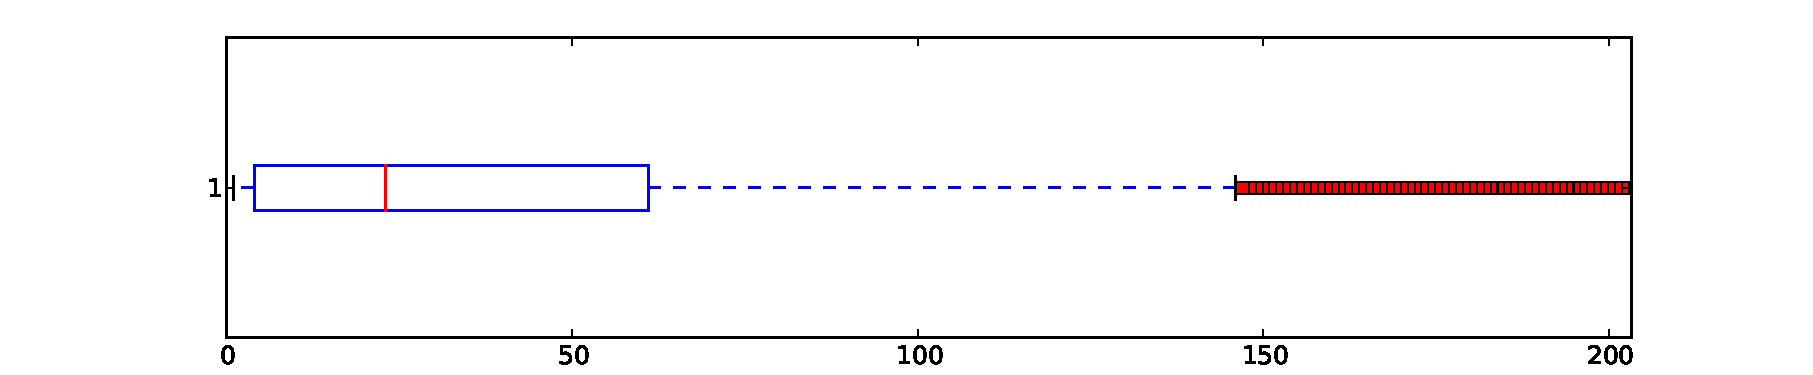
\includegraphics[width=0.9\textwidth]{Figures/boxplot_events.pdf}}
\caption{A boxplot visualizing the Events distribution incorporating the five number summary.}
\label{fig:boxplot_events}
\end{figure}

The two lines outside the box in Figure~\ref{fig:boxplot_events} are called whiskers and represent the extreme low and high values that are less than $1.5 \times IQR$ beyond the quartiles. The first and third quartiles represent the ends of the box and the median is the red line. The red \textit{squares} are individual points called \textit{outliers}. Only about $6\%$ or $\approx 5500$ players of the entire population generated more than 150 events, $0.3\%$ or $\approx300$ players have more than 1000 events and less than ten people have a range of $5.000-10.000$ generated events! A histogram showing the frequency of events generated by players is shown in Figure~\ref{fig:histogram_events_iqr}, zooming in on the spread that gives the range covered by the middle half of the data.

\begin{figure}[here]
\centerline{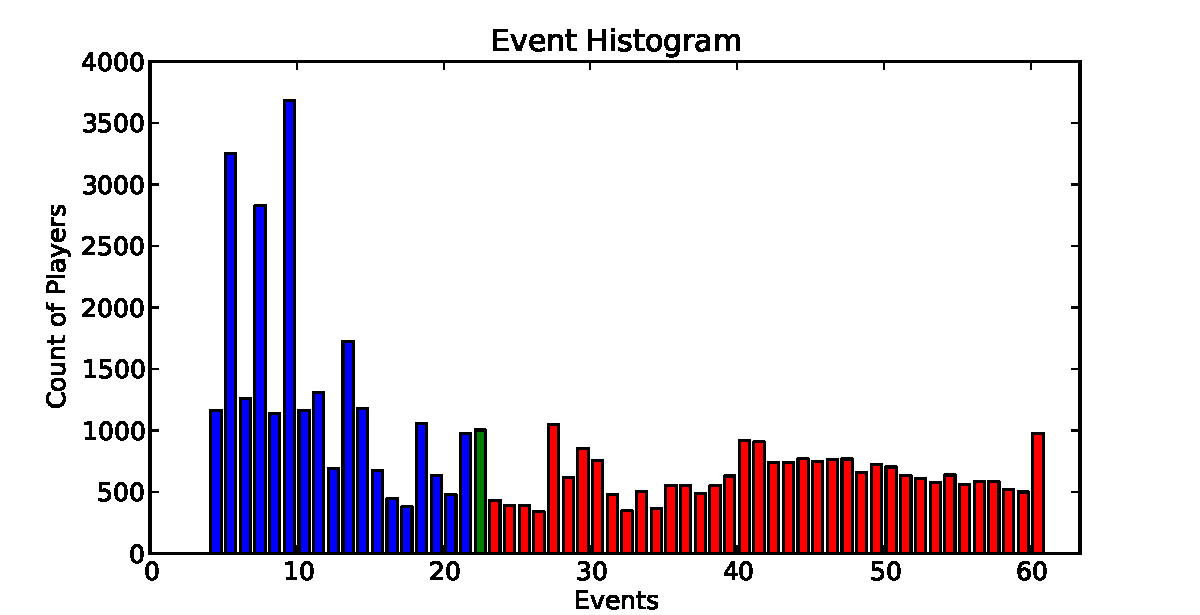
\includegraphics[width=0.9\textwidth]{Figures/histogram_events_iqr.pdf}}
\caption{A histogram for number of events using singleton buckets in the interquartile range (IQR) defined as $Q3 - Q1$, range covered by the middle half of the data.}
\label{fig:histogram_events_iqr}
\end{figure}


\subsection{Game Metric Construction}
\label{gamemetric}
For this thesis we tried to keep the number of game features in minimal and decided to build our feature vector with three features. Given the limited knowledge and information that we have about individual events we decided to select events that have high frequency compared to other events and hopefully could describe different behaviors between groups of players in those features. A $3-dimensional$ feature vector was constructed for each unique player, containing a frequency of three events generated by the player. The aggregated events are:
\begin{itemize}
\item Login: Number of logins/access into different areas in the game($\mu = 2.4, \sigma = 4.8$)
\item Battle: Number of battles this player have started ($\mu = 3.7, \sigma = 9.6$)
\item Premium Spending: Number of times this player spends a in-game money on virtual items or resources ($\mu = 1.1, \sigma = 2.7$) 
\end{itemize}

The five number summary of the skewed distribution is in Table~\ref{tab:FiveSummaryLoginsBattlesPremium}. Boxplots visualizing the distributions for these events are shown in relevant figures below, Logins in Figure~\ref{fig:boxplot_logins}, Battles in Figure~\ref{fig:boxplot_battles} and Premium spent events in Figure~\ref{fig:boxplot_premium}.


\begin{table}[h]
\centering
\begin{tabular}{| l | l | l | l | l | l |}
    \hline
    & \textit{Min} & $Q_1$ & \textit{Median} & $Q_3$ & \textit{Max} \\ \hline
    Logins & 0 & 1 & 1 & 2 & 220 \\ \hline
    Battles & 0 & 0 & 1 & 4 & 439 \\ \hline
    Premium spent & 0 & 0 & 0 & 1 & 100 \\ \hline
\end{tabular}
\caption{This table shows the five number summary for the Logins, Battles and Premium spent events generated by each unique player in the dataset.}
\label{tab:FiveSummaryLoginsBattlesPremium}
\end{table}

The features values are spread out over large range of values, in the preprocessing Section~\ref{preprocessing} we explain how we detect and remove the outliers or anomalies from our data before we apply our MR k-means algorithm using a \textit{z-score} method.

\begin{center}
\begin{figure}[h]
\centerline{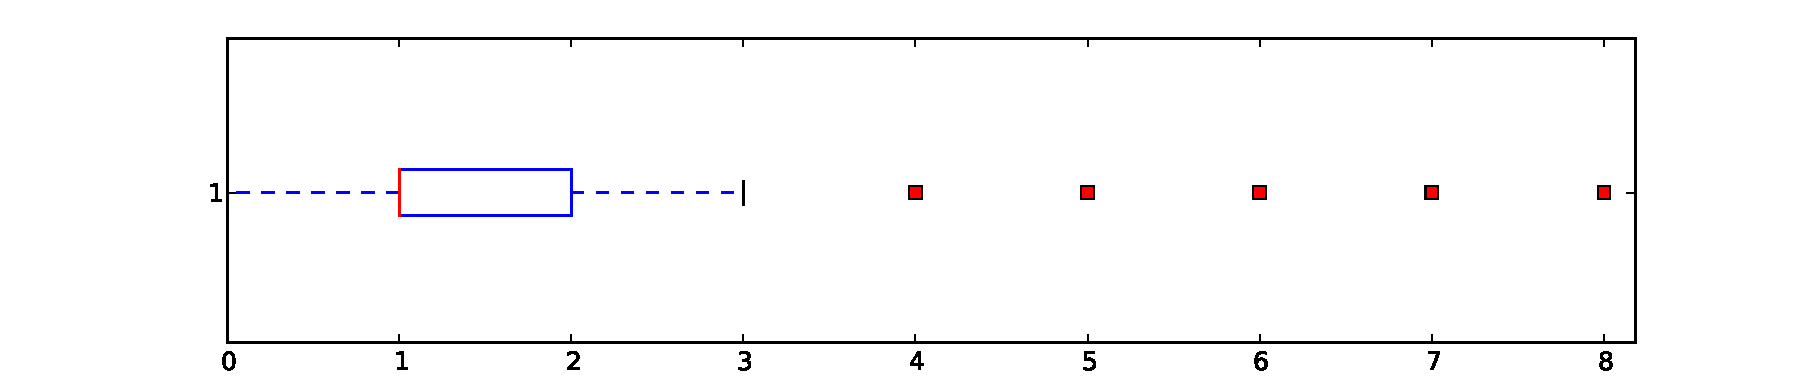
\includegraphics[width=0.9\textwidth]{Figures/boxplot_logins.pdf}}
\caption{A boxplot visualizing the Login events distribution incorporating the five number summary.}
\label{fig:boxplot_logins}
\end{figure}

\begin{figure}[h]
\centerline{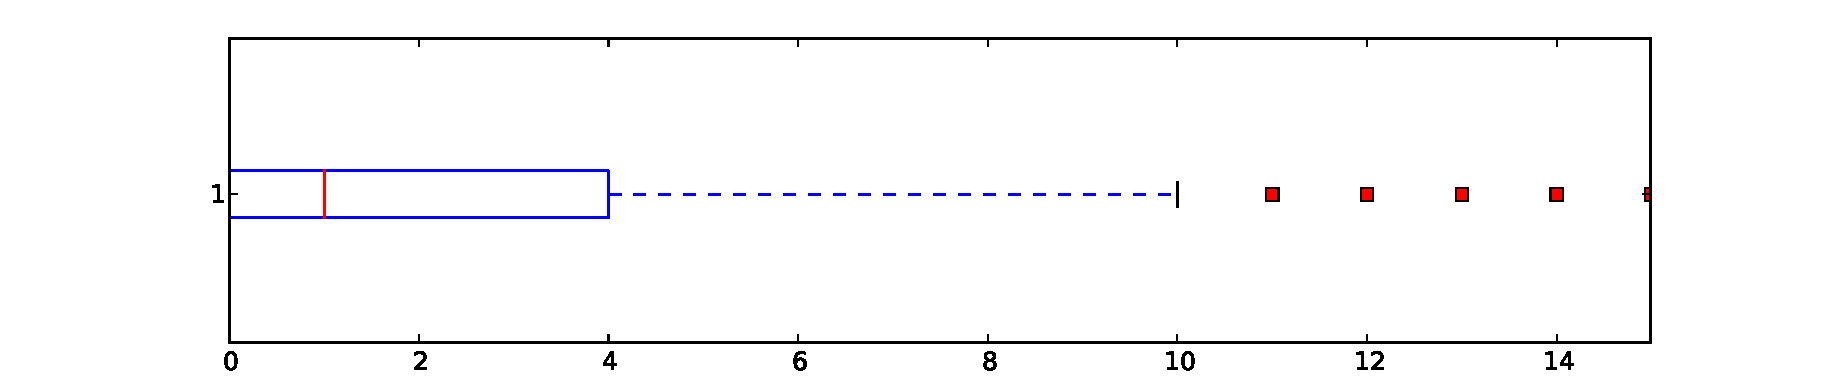
\includegraphics[width=0.9\textwidth]{Figures/boxplot_battles.pdf}}
\caption{A boxplot visualizing the Battle events distribution incorporating the five number summary.}
\label{fig:boxplot_battles}
\end{figure}

\begin{figure}[here]
\centerline{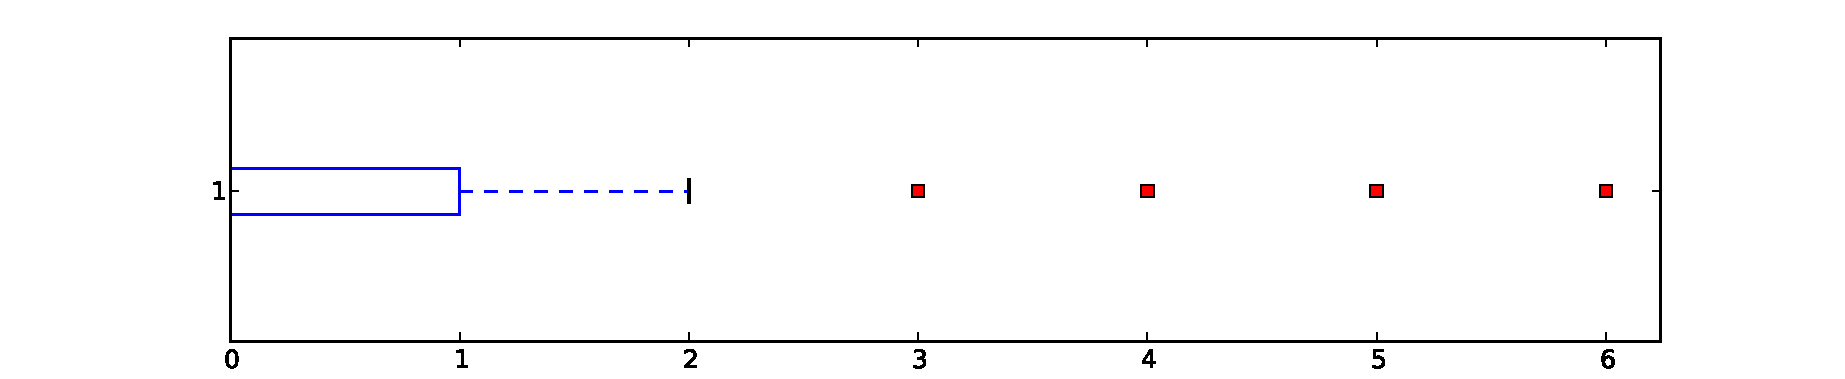
\includegraphics[width=0.9\textwidth]{Figures/boxplot_premiumspent.pdf}}
\caption{A boxplot visualizing the Premium spent events distribution incorporating the five number summary.}
\label{fig:boxplot_premium}
\end{figure}
\end{center}


\subsection{Preprocessing}
\label{preprocessing}
User telemetry from games can be very noisy in that sense it can contain lots of irrelevant events and logging information and even developers from the game studio can generate events. For this dataset this we performed several preprocessing steps:
\begin{itemize}
\item Sort the events after event timestamp.
\item Split the dataset into $10$ approx. equally sized data set pieces.
\item Filter out irrelevant events and logging information. E.g. Events not origin from Facebook or Google Plus, non related events and in game studio debugging generated events.
\item For each data set piece:
 \begin{itemize}
 \item Counting the events mentioned above per user to build our feature vector.
 \item Remove outliers or anomalies from the data.
 \item Standardize the data to standard scores also called \textit{z-score}. Transforming the data
to standard normal distribution, with $\mu = 0$ and $\sigma = 1$. 
 \end{itemize}
\end{itemize}

To apply our incremental MR k-means algorithm we need to have multiple batches of data to process incrementally. We use the real game dataset that we got from GA and split it up into $10$ equally sized data batches sorted after the event arrival timestamp. By doing so we try to simulate that we are processing multiple batches of data in the same order as the events were generated over mulitple time-periods or days, like at GA. Next we filter out irrelevant information, e.g. information that don't contribute as a event logging or are obviously from the game designers themselves.

When processing each data batch we aggregate or count the events that we selected before to build our feature vector for each unique player in the data set. Next we find the outliers by transforming the data to standard scores using the \textit{zero mean normalization} (ZMN), also called \textit{z-score}, with standard normal distribution having zero mean and unit variance $\mu = 0$ and $\sigma = 1$. A feature vector that has a feature value z-score that is more than $3$ standard deviations away from the mean is considered an outlier in the data and is removed from the original data batch. Having a data batch without outliers we now can transform the data again using ZMN, without having the outliers to effect our transformation. The ZMN is defined as follows


\begin{center}
$z = \dfrac{x  - \mu}{\sigma}$ 
\end{center}


Using ZMN is widely used in machine learning algorithms and is needed when calculating the distance between two points (feature vectors) such that each feature contributes approximately equally to the final distance.

Removing the outliers from the whole dataset, using the ZMN method described above, the total number of unique players become approx $90.800$ instead of approx. $94.000$, removing $\approx 4\%$ of the population. The five number summary for the whole dataset can be found in Table~\ref{tab:FiveSummaryLoginsBattlesPremiumWoOutliers}, notice the range of values compared to the Table~\ref{tab:FiveSummaryLoginsBattlesPremium} in Section~\ref{gamemetric}. The multiple data batches that we feed into our clustering algorithm had $\approx 5\%$ player feature vectors removed on average, see Table~\ref{tab:DatabatchesWoOutliers} below.

\begin{table}[h]
\centering
\begin{tabular}{| l | l | l | l | l | l |}
    \hline
    & \textit{Min} & $Q_1$ & \textit{Median} & $Q_3$ & \textit{Max} \\ \hline
    Logins & 2 & 1 & 1 & 2 & 16 \\ \hline
    Battles & 0 & 0 & 1 & 4 & 32 \\ \hline
    Premium spent & 0 & 0 & 0 & 0 & 9 \\ \hline
\end{tabular}
\caption{This table shows the five number summary for the Logins, Battles and Premium spent events generated by each player from the whole dataset with outliers removed.}
\label{tab:FiveSummaryLoginsBattlesPremiumWoOutliers}
\end{table}


\begin{table}[h]
\centering
\scalebox{0.8}{%
\begin{tabular}{| l | l | l | l | l | l | l | l | l | l | l |}
    \hline
    & Data 1 & Data 2 & Data 3 & Data 4 & Data 5 & Data 6 & Data 7 & Data 8 & Data 9 & Data 10 \\ \hline
    Players & 14054 & 13365 & 13403 & 13503 & 13441 & 13276 & 12839 & 13413 & 13473 & 13412 \\ \hline
    Outliers  & 658 & 741 & 661 & 673 & 748 & 698 & 685 & 724 & 669 & 680 \\ \hline
    $\%$ removed & $4,68\%$ & $5,44\%$ & $4,93\%$ & $4,98\%$ & $5,56\%$ & $5,25\%$ & $5,33\%$ & $5,39\%$ & $4,96\%$ & $5,07\%$ \\ \hline
\end{tabular}}
\caption{This table shows the player population, number of outliers found and the percentage of the population removed, for each data batch.}
\label{tab:DatabatchesWoOutliers}
\end{table}



\section{K-means algorithm in MapReduce}
\textit{TODO Describe the k-means algorithm implementation in MapReduce and the relevant pseudo codes and pictures}


A k-means algorithm was implemented in MapReduce that is able to process large-scale datasets. We started to implement a simple version of k-means that assigns each point to a nearest cluster in the \textit{Map} function and calculates the new centroid in the \textit{Reduce} phase. Next version had a \textit{Combiner} implemented that performs a reduce work on the same computer node as the Mapper, by calculating intermediate sums of all points for each cluster from a Map function. This minimizes the data needed to be transferred and shuffled by the MapReduce framework to the Reducer, only sending an intermediate sum with each cluster centroid from each mapper instead of list of all points in each cluster [REFERENCE]. The final k-means version uses a more efficient way of calculating the distance to the nearest centroid for each point. Using a matrix calculation that returns a distance matrix that represents distances from all points to all centroids. These different versions are compared below in respect to time and space complexity.


\subsection{K-means - Map and Reduce version}
\lipsum[1]

\subsubsection{Map}
\textit{TODO Describe the map function}

\lipsum[1-2]


\subsubsection{Reduce}
\textit{TODO Describe the Reduce function}

\lipsum[7-8]

\subsection{K-means - Map, Combine and Reduce version}
\lipsum[1]

\subsubsection{Combine}
\textit{TODO Describe the Combine function}

\lipsum[5-6]

\subsection{K-means - Efficient version}
\lipsum[1]

\subsubsection{Map}
\textit{TODO Describe the map function}

\lipsum[1-2]

\subsubsection{Combine}
\textit{TODO Describe the Combine function}

\lipsum[5-6]


\subsubsection{Reduce}
\textit{TODO Describe the Reduce function}

\lipsum[7-8]


\subsection{Distance measure}
\textit{TODO Describe the distance measure used in k-means}

\lipsum[1]


\section{MapReduce Development Environment}
\textit{TODO Describe the set-up for the experiments}
The MapReduce k-means algorithm was implemented using a framework called \textit{mrjob}~\footnote{http://pythonhosted.org/mrjob/}. Mrjob is a open-source Python framework actively maintained by Yelp~\footnote{http://opensource.yelp.com/}, that allows MapReduce jobs to be written in Python 2.5+ and executed on several platforms. Using mrjob allows for rapid implementation of MapReduce jobs by running them locally for development purposes and easily run them on your own Hadoop cluster or using the Amazon Elastic MapReduce (Amazon EMR)\footnote{http://aws.amazon.com/elasticmapreduce/}. Amazon EMR is a web service that allows developers to buy time on a Hadoop cluster to process large-scale data easily and cost-effectively.

The Python programming language was chosen for this study because GameAnalytics (GA) also uses Python and mrjob to implement their MapReduce jobs. Allowing GA easily to use and build further on the implementation from this study. 
\lipsum[1-3] % Methodology

% Chapter 5

\chapter{Results and Discussion} % Write in your own chapter title
\label{Chapter5}
\lhead{Chapter 5. \emph{Results and Discussion}} % Write in your own chapter title to set the page header

\section{Results}
\textit{TODO Show results with relevant pictures and what they mean}

\lipsum[1-5]


\section{Discussion}
\textit{TODO Describe the results with more detailed explanations}

\lipsum[1-2] % Results and Discussion

% Chapter 6

\chapter{Discussion} % Write in your own chapter title
\label{Chapter6}
\lhead{Chapter 6. \emph{Discussion}} % Write in your own chapter title to set the page header

The MapReduce k-means clustering algorithm in this thesis found general player behaviour in a multiple batches of real game data. Results showed quality and stable clusters, the algorithm used efficient MR strategies by implementing a Combiner phase to reduce traffic and efficient vectorisation operations computing the nearest centroid in the Mapper phase. Scalable both horizontal and vertical using Amazon EMR, running multiple on-demand instances on a Hadoop cluster.

The algorithm clusters each data batch $n$-iterations resulting in centroids describing the a general player behaviour of each cluster, and incrementally clusters next incoming data batches by using the output from the previous batch as input to the next batch. So each data batch contributes to the general player behavior for the next batch. 

Iterating only once per game data batch with the MR k-means algorithm resulted in higher quality and more stable clusters than increasing the number of iterations per batch. Allowing the centroids move slowly beetween different data batches, instead taking aggressive steps towards a data that will change in the next batch.

Three player profiles were interpreted from the last game data batch, using the centroids of the clusters to describe the general player behaviours, after incrementally clustering the previous data batches. These player profiles were not evaluated by a game developer that developed the game under research but instead it was evaluated using the authors intuition.

Evaluating the algorithm on a fictive dataset gave interesting results, where there was completely different behaviour, but was a fictive one. Three clusters are on a aggressive move and changes every data batch was a little bit more challence. The Iteration $2$ version was ranked highest in cluster quality and error stability, but Iteration $1$ was not far way. 

The weakness for the algorithm is that it was not evaluated on larger multiple set of data batches, both in numbers and volume. Such that these results just indicate that for a real game data and a similar game it would be good to use one iteration and slowly after incrementally processing multiple batches the centroids will give high quality clusters and give a good representation of the general behaviors of the population. Also the $k$ number of clusters to be found by k-means was not tested with different numbers than $3$, this would be ofcourse be problem specific. Also interesting is to have the $k$ to adjust to evolving behaviors in the data. Looking into iterative MapReduce frameworks where there is possible to run $n$ iterations inside MapReduce instead of launching a MapReduce job each time (more overhead), would be a good research.

The MR k-means algorithm can be applied to any game data and scales out when increasing the dataset size. % Conclusions

%% Chapter 7

\chapter{Conclusions} % Write in your own chapter title
\label{Chapter7}
\lhead{Chapter 7. \emph{Conclusions}} % Write in your own chapter title to set the page header

Data is all around us and is inevitable, it has been around for a quite some time but is getting bolder and more complex to understand and work with. Using services like Amazon Elastic MapReduce web service and their simple web storage (S3) is a right step analyzing and understanding these gigantic volumes of data. Implementing algorithms that can be distributed and executed in parallel is a very powerful tool when using it on large-scale data. 

Free online games (Free-to-Play) are increasing each day through, e.g. Facebook and Google Plus, generating revenue through in-game transactions. Data analysis and better understanding the customers and their player behaviour is a vital information to keep the customer in the game and to buy more virtual items using micro-transactions with real money. The games can be very complex and offer wide range of events and behaviour where millions of users interact to each other.

The goals for this thesis were achieved and the contribution are the following:
\begin{itemize}
	\item A MapReduce k-means algorithm that can find general player behaviour in the real game data set provided by GameAnalyltics, by incrementally cluster multiple batches. And were interpreted to player profiles.
	\item The algorithm finds stable and quality clusters while incrementally clustering multiple data batches, both for real game data and fictive generated datasets, where centroids move rapidly between batches.
	\item The algorithm uses an efficient MR implementation function called Combiner, to minimize network and data traffic inside the MapReduce framework.
	\item The algorithm uses efficient computation vectorisation approaches to perform fast operations on array like data objects, when computing the nearest centroid in the Mapper phase inside MR.
\end{itemize}



\subsection{Future Work}
\begin{itemize}
	\item Evaluate the algorithm over larger time periods, more number of data batches and in larger size and for different real life datasets. Interesting would to see if the algorithm continues to be stable.
	\item Evaluate which number of iterations would give the best results to certain types of evolving datasets.
	\item Looking into Iterative MapReduce frameworks that are much more efficient to deal with many iterations, by running a internal loop, meaning a separate control program is redundant.
	\item Evaluate if there is a possibility to use a distance matrix computation efficiently to find the nearest centroid running on Amazon EMR, without running into memory troubles. E.g. using more powerful \textit{Master Controller} instance, or higher memory instance running on Hadoop.
\end{itemize}
 % Conclusion

%% ----------------------------------------------------------------
% Now begin the Appendices, including them as separate files

\addtocontents{toc}{\vspace{2em}} % Add a gap in the Contents, for aesthetics

\appendix % Cue to tell LaTeX that the following 'chapters' are Appendices

% Appendix A

\chapter{Appendix Title Here}
\label{AppendixA}
\lhead{Appendix A. \emph{Appendix Title Here}}

Write your Appendix content here.	% Appendix Title

%\input{./Appendices/AppendixB} % Appendix Title

%\input{./Appendices/AppendixC} % Appendix Title

\addtocontents{toc}{\vspace{2em}}  % Add a gap in the Contents, for aesthetics
\backmatter

%% ----------------------------------------------------------------
\newcommand*{\doi}[1]{\href{http://dx.doi.org/\detokenize{#1}}{doi: \detokenize{#1}}}
\label{Bibliography}
\lhead{\emph{Bibliography}}  % Change the left side page header to "Bibliography"
\bibliographystyle{unsrtnat}  % Use the "unsrtnat" BibTeX style for formatting the Bibliography
\bibliography{Bibliography}  % The references (bibliography) information are stored in the file named "Bibliography.bib"

\end{document}  % The End
%% ----------------------------------------------------------------